\section{Hierarchical clustering with mixed-type variables }

\subsection{Problem}
One important aspect of processing information is to deal with different types of data, because not every attribute is of the same nature. 

Given an example: A survey is conducted about a person’s daily life. The considered factors are: Age, Gender, Job, and how Satisfactory they are. A quick observation shows that these values are not the same type. Age is measured in integer, which is a numerical value; Gender can be used as a binary value, with 0 (false) being female, and 1 (true) being male; Job is shown with many options (engineer, businessman, storekeeper, homemaker, …), therefore it is a nominal value; and a scale of 1 to 10 to rate the person’s satisfaction, which is an ordinal value. This is just some common types of data that we usually deal with, so knowing how to process mixed data can benefit us with a more realistic model.

This section will discuss Gower’s Distance, which is one of the methods to deal with this problem. 

\subsection{Gower's Distance}
Gower’s Distance is a method for computing distances between two data points. The strength of this method comes from the fact that it is usable for other types of data beside numerical, which is more flexible than the common methods (Euclidean distance, Manhattan distance, …). Another advantage is that Gower’s Distance scales the ranges of data into between 0 and 1, with addition of allowing a user-defined weighting scheme. But for this project, an unweighted model is constructed. 

The basic calculation of Gower’s Distance is as follow. Data will be separated into two types: numerical and non-numerical.

With numerical, we can compute the data by the formular: 

    \quad |Difference| / Range

    \begin{itemize}
        \item Difference = Data[i] - Data[i+1] ; 
        \item Range is the difference between the maximum and the minimum data points. 
    \end{itemize}

With non-numerical values, we can compute by compare the data points. If they are identical, the distance will be 0, if not then the distance will be 1.

There are some packages that uses or have the option for Gower’s calculation, and in this project "cluster" package is used, which contains function "daisy" that allows Gower as an option.

\subsection{Code Explaination}
(Source code link: \url{https://github.com/vhtuananh020402/Group4_Data_analysis/blob/main/completed_gower_ward.r})

\vspace{1mm}
First, libraries and data frame will be imported. The function na.omit(df) is necessary for omitting missing values in the data frame.
    \begin{code}{R}
        library(factoextra)   # clustering visualization
        library(ggplot2)      # draw distribution graph

        # read data frame
        df <- read.csv("data/clean_data_v2.csv")
        # remove missing values in data frame
        df <- na.omit(df)
    \end{code}
Then, data will be processed by splitting into 3 types: numerical, nominal, and ordinal. Nominal is defined by using function lapply(df[nom\textunderscore attr], as.factor) to change value type into factor. Ordinal is defined by using function factor(), which has the option order = TRUE, and level is from lowest to highest. Finally, process\textunderscore dataset will contain the complete dataset for analysing steps.
    \begin{code}{R}
            # --- Data Preparation --- #
        # add into numerical value
        num_attr <- c("Age")

        # add into nominal value
        nom_attr <- c("Field", "Genre", "Factor")
        df[cat_attr] <- lapply(df[cat_attr], as.factor)

        # add into ordinal value
        ord_attr <- c("Frequency")
        df$Frequency <- factor(df$Frequency, 
                                    order = TRUE, 
                                    level = c("Less than 2 hours", 
                                                "2 - 5 hours", 
                                                "6 - 10 hours", 
                                                "11 - 15 hours", 
                                                "16 - 20 hours", 
                                                "More than 20 hours"))

        # put everything into a complete data set
        process_dataset <- df %>% select(num_attr, ord_attr, cat_attr)

        head(process_dataset)
    \end{code}
Function daisy() will calculate the dissimilarity matrix, with process\textunderscore dataset as input, and gower  is used as the calculation metric. After that, the hierarchical clustering model is built using hclust() function. Clustering method ward.D is chosen because it brings the best result when plotting dendrogram.
    \begin{code}{R}
            # --- Calculation --- #
        # calculate Gower's distance
        gower_dist <- daisy(process_dataset, metric="gower")   

        # hierarchical clustering, using ward.D method 
        gower_hcl <- hclust(gower_dist, method = "ward.D")  

            # --- DENDROGRAM ---- #
        # plot dendrogram
        plot(gower_hcl, cex = 0.6)

        # draw borders for the individual clusters
        rect.hclust(gower_hcl, k = 7, border = 2:7)
    \end{code}
Histograms are used to present the distribution of each attribute in each cluster. “k” represents the number of clusters that we want. The decision k = 7 is made according to the previous method of building hierarchical clustering using Dummy Variable. For some unknown reasons, the functions that find the optimal number of clusters is unusable in this section.
    \begin{code}{R}
            # --- HISTOGRAM --- #
        # cut into k clusters
        k <- 7
        clusters <- cutree(gower_hcl, k)

        # add the cluster assignments to the data frame
        df\$Cluster <- factor(clusters)

        # histogram of Genre distribution in each cluster
        ggplot(df, aes(x = Genre)) +
            geom_histogram(stat = "count", fill = "lightblue", color = "black", linewidth = 0.8) +
            facet_wrap(~ Cluster) +
            theme(axis.text.x = element_text(angle = 45, hjust = 1)) +
            labs(title = "Genre Distribution in Each Cluster", x = "Genre", y = "Count")

        # histogram of Field distribution in each cluster
        ggplot(df, aes(x = Field)) +
            geom_histogram(stat = "count", fill = "red", color = "black", linewidth = 0.8) +
            facet_wrap(~ Cluster) +
            theme(axis.text.x = element_text(angle = 45, hjust = 1)) +
            labs(title = "Field Distribution in Each Cluster", x = "Field", y = "Count")

        # histogram of Factor distribution in each cluster
        ggplot(df, aes(x = Factor)) +
            geom_histogram(stat = "count", fill = "lightgreen", color = "black", linewidth = 0.8) +
            facet_wrap(~ Cluster) +
            theme(axis.text.x = element_text(angle = 45, hjust = 1)) +
            labs(title = "Factor Distribution in Each Cluster", x = "Factor", y = "Count")

        # histogram of Age distribution in each cluster
        ggplot(df, aes(x = Age)) +
            geom_histogram(stat = "count", fill = "orange", color = "black", linewidth = 0.8) +
            facet_wrap(~ Cluster) +
            theme(axis.text.x = element_text(angle = 45, hjust = 1)) +
            labs(title = "Age Distribution in Each Cluster", x = "Age", y = "Count")

        # histogram of Frequency distribution in each cluster
        ggplot(df, aes(x = Frequency)) +
            geom_histogram(stat = "count", fill = "darkgrey", color = "black", linewidth = 0.8) +
            facet_wrap(~ Cluster) +
            theme(axis.text.x = element_text(angle = 45, hjust = 1)) +
            labs(title = "Frequency Distribution in Each Cluster", x = "Frequency", y = "Count")
    \end{code}

\subsection{Results}
    \subsubsection{Dendrogram}
        The dendrogram shows the relations between all of the observations, with each cluster is shown by colored lines. With many tries and many different methods, we decided to keep this result because this is more evenly distributed model than other versions.
        \begin{figure}[H]
            \centering
            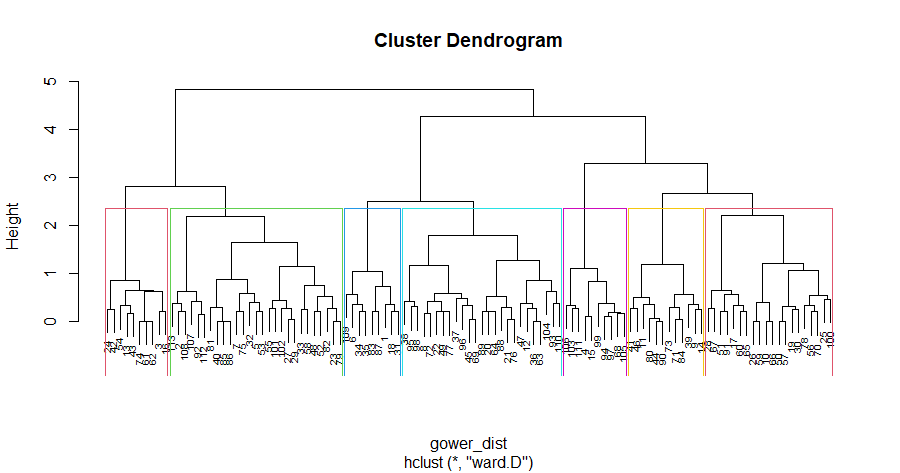
\includegraphics[scale=0.6]{graphics/gower/dendrogram/gower_dist_ward.png}
            \caption{Result visualized by Dendrogram}
        \end{figure}
    \subsubsection{Histograms and observing patterns}
        We only obverse the histograms of the following attributes: Age, Genre, Field, Frequency and Factor. Gender and Platform are useful for unifying the dataset, but those are not considered to be the attribute that contributing to the recommended system in real-world practices. Therefore, we omit them when graphing the histograms.
        \begin{figure}[H]
            \centering
            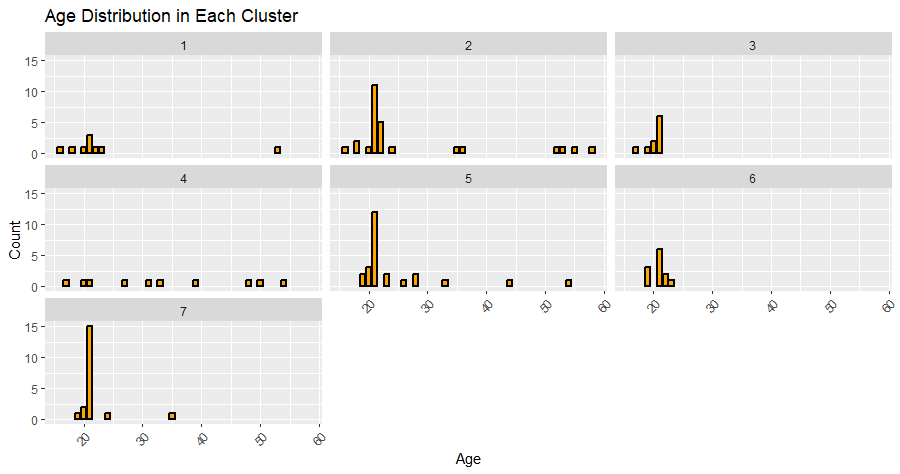
\includegraphics[scale=0.6]{graphics/gower/histogram/age distrib.png}
            \caption{Age distribution in each cluster visualized by Histogram}
        \end{figure}
        \begin{figure}[H]
            \centering
            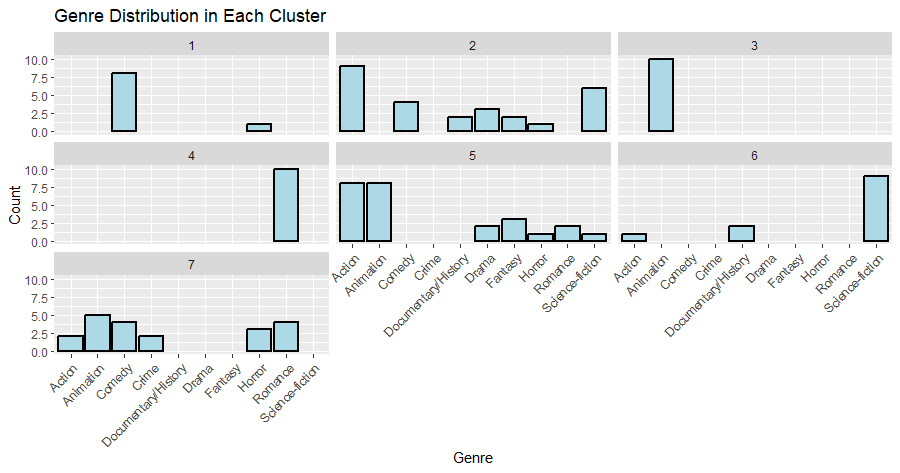
\includegraphics[scale=0.6]{graphics/gower/histogram/genre distrib.png}
            \caption{Genre distribution in each cluster visualized by Histogram}
        \end{figure}
        \begin{figure}[H]
            \centering
            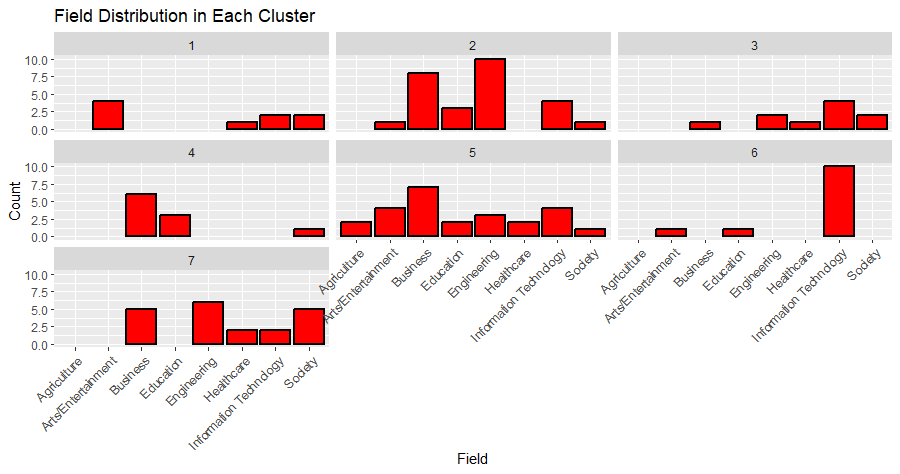
\includegraphics[scale=0.6]{graphics/gower/histogram/field distrib.png}
            \caption{Field distribution in each cluster visualized by Histogram}
        \end{figure}
        \begin{figure}[H]
            \centering
            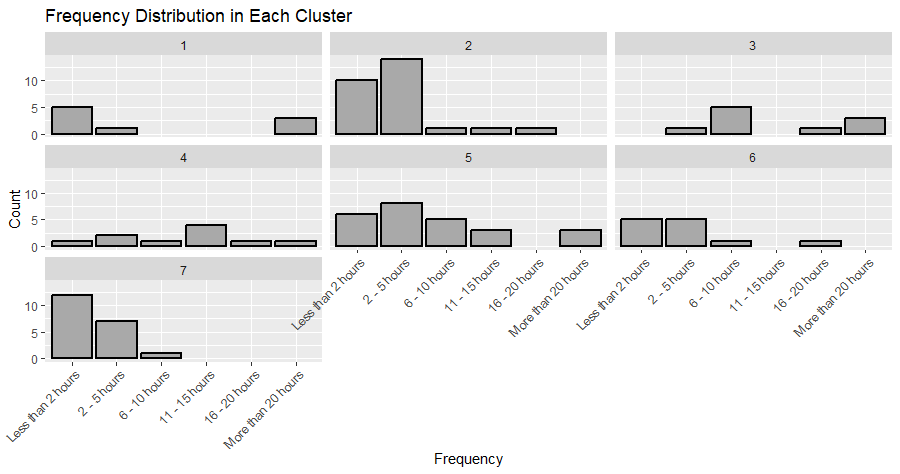
\includegraphics[scale=0.6]{graphics/gower/histogram/freq distrib.png}
            \caption{Frequency distribution in each cluster visualized by Histogram}
        \end{figure}
        \begin{figure}[H]
            \centering
            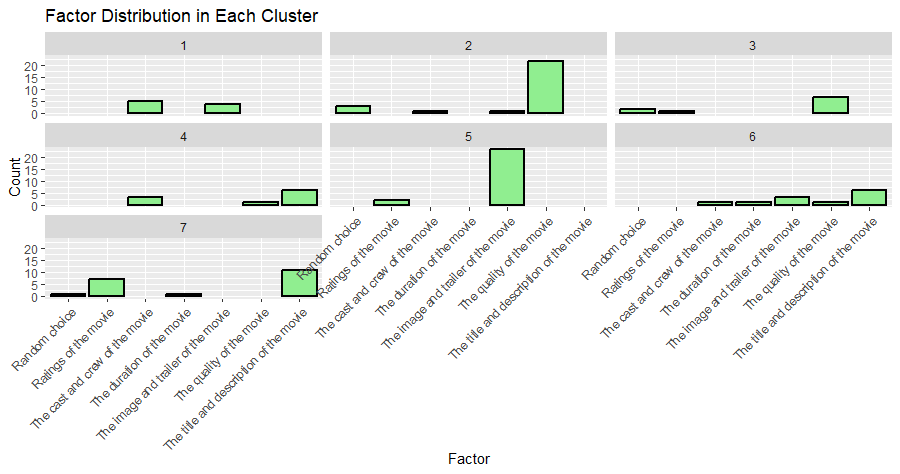
\includegraphics[scale=0.6]{graphics/gower/histogram/factor distrib.png}
            \caption{Factor distribution in each cluster visualized by Histogram}
        \end{figure}
The followings are concluded from the histogram for each cluster:
\newline

Cluster 1: Mostly from under 25 years old. Comedy is the most watched genre, with watching time falls between “Less than 2 hours” and “Over 20 hours”. Art/Entertainment field being the highest choice here, with IT and Society being the lesser. “Cast/Crew” and “Image/Trailer” are the reasons for choosing and watching.
\newline

Cluster 2: The majority are 21 years old, with Action and Sci-fi are the most viewed. Comedy, Documentary/History, Drama, Fantasy and Horror are also considered. Watching time is from 2 to 5 hours. They are largely come from Engineering and Business. “Quality” is the most important factor for picking movies.
\newline

Cluster 3: The majority is 21 years old, with Animation being the only choice for genre. “6 - 10 hours” and “more than 20 hours” are the standout choices. Engineering, IT and Society are evenly distributed fields, with IT being the highest choice. “Quality” is the most important factor.
\newline

Cluster 4: Ages are evenly distributed across the range. Romance is the only viewed genre here. Watching time is varied, with “11 – 15 hours” being the highest choice. Business is the most picked field here, and they consider “Cast/Crew” and “Title/Description” when choosing movies.
\newline

Cluster 5: Mostly 21 years old, with Action and Animation are the highest viewed genre here, also with somewhat evenly distributed between Drama, Fantasy, Romance. Watching time is largely from “Less than 2 hours” to “6 – 10 hours” range. Business is the most choice for field, but the occupation is distributed across the range. “Image/Trailer” is the most important factor.
\newline

Cluster 6: Around 20 years of age. Science-fiction is the most viewed genre, with a small percentage coming from Action and Documentary/History. Mostly from “Less than 2 hours” to “2 - 5 hours” range of watching time. The IT field is the highest choice, with “Image/Trailer” and “Title/Description” are the most important factor. 
\newline

Cluster 7: The majority are 21 to 22 years old. Action, Animation, Comedy, Crime, Horror and Romance shared the genre distribution without much differences. Watching periods mostly come from “Less than 2 hours” to “2 – 5 hours” range. Business, Engineering and Society are the most choices for field of occupation, and “ratings” as well as “title/description” are the most important factors.

\subsection{Shortcomings}
With the lack of documentation, using libraries that implement Gower’s Distance is complicated and troublesome, as it leads to unexpected errors. One example is that functions to find the optimal number of clusters cannot be applied, whether it is Elbow, Silhouette or Gap Statistic method. Because of the limited time frame of this project, the errors cannot be solved yet. Therefore, it is crucial to research thoroughly beforehand if using the existing libraries for this method.